\chapter{Implementation}
When talking about software development processes, there is always an implementation phase which is the stage that the actual coding takes place, in respect to the earlier design phase. Modular development is not an exception, this stage of modular development is the so called {\bf modular programming} and this stage will make use of the modelings made in the previous chapter to implement the {\bf eye droid} system.

In this chapter, only the core part of the system will be discussed, code listings will be provided to show how this system was implemented. Since this development was done for the android platform using the native android language and Kivy framework, Java programming language will mostly be used and in a later module Python programming language.

Modular development approach is the target approach for developing this software system, as such, the package feature of the java language was used to divide the application into modules and also with one module which is an application level module.

\section{I/O Module}
The {\bf input and output module} is a package which consists of a single class {output.java} this module handles all the I/O operations that is needed in this particular software. Within the class, three methods have been developed to handle saving files on the device's local storage, files such as images (.jpeg, .png e.t.c) and text files. The three methods include ({\it saveFrame(Bitmap), writeToFile(String), saveFace(Bitmap)}) all this methods contain the same structure and differ only by storage destinations and type of files, in which case, one method is sufficient to understand this module. 

\begin{lstlisting}[label=Saving-a-file-in-device-storage-drive,caption=Saving files in device storage drive]
public void saveFace(Bitmap image) {
	try {
		String root = Environment.getExternalStorageDirectory().toString();
		File dir = new File(root + "/org.plaix.viewer/Images");
		dir.mkdirs();
		Date date = new Date();
		CharSequence sequence = DateFormat.format("MM-dd-yy-h-mm-ss",
				date.getTime());
		String imageName = "Image-" + sequence + ".jpg";
		path = root +"/org.plaix.viewer/Images/"+imageName;
		File file = new File(dir, imageName);
		FileOutputStream fos;
		fos = new FileOutputStream(file);
		image.compress(Bitmap.CompressFormat.JPEG, 90, fos);
		fos.close();
	} catch (FileNotFoundException e) {
		e.printStackTrace();
	} catch (IOException e) {
		e.printStackTrace();
	}

}
\end{lstlisting}

Listing 6.1 shows the method {\it saveFace()} which takes a single parameter of type {\it Bitmap}, gets the path to the devices's local storage with the method {\it Environment.getExternalStorageDirectory()}, creates a file(directory) and concatenate the root directory with the directory in which the file is to be saved to. After creating the file, a name for the file is generated, a {\it FileOutputStream} object is created with the file and the image is compressed into a JPG format using the method {\it Bitmap.compress()} with parameters of the format and the file output stream.

\newpage
\section{Database Module}
The {\bf database module} contains two java classes, one is an implementation of the relational model of the database (LogModel.java) describing the structure of the database. The second class (LogHelper.java) is the implementation of the {\it SQLiteOpenHelper} which is a helper class to manage the creation, opening, upgrading and versioning of the database.  

\begin{lstlisting}[label=database-relational-model,caption=Relational Model of the Database Module]
public class LogModel {
	private long id;
	private String date;
	private String comment;
	
	public LogModel(){}
	
	public LogModel(long id, String date, String comment){
		this.id = id;
		this.date = date;
		this.comment = comment;		
	}
	
	...
	
	@Override
	public String toString(){
		return id+". "+date+": "+comment;
	}
	
}
\end{lstlisting}

From the code listing above (listing 6.2) it is easy to deduce the structure of the database having a single table with the columns {\it id, date and comment}, also having two constructors for instantiating the model object, one taking no arguments and the other taking three arguments each being a column in the table. This is also accompanied by a set of {\it getters and setters}. The {\it toString()} method was overridden to return the columns in the desired format as shown in the listing.
\newpage
\begin{lstlisting}[label=sqlite-helper,caption=Implementaion of the SQLiteOpenHelper] 
	...
	
	public LogHelper(Context context, String date, String comment){
		super(context, DATABASE_NAME, null, DATABASE_VERSION);
		this.date = date;
		this.comment = comment;
	}
	
	public LogHelper(Context context){
		super(context, DATABASE_NAME, null, DATABASE_VERSION);
	}
	
	@Override
	public void onCreate(SQLiteDatabase database) {
		database.execSQL(CREATE_DATABASE);
	}

	@Override
	public void onUpgrade(SQLiteDatabase database, int oldVer, int newVer) {
		database.execSQL("DROP TABLE IF EXISTS " + TABLE_LOG);
		onCreate(database);
	}
	
	public void insertComment(){
		SQLiteDatabase db = this.getWritableDatabase();
		ContentValues values = new ContentValues();
		values.put(DATE_COLUMN, date);
		values.put(COMMENT_COLUMN, comment);
		db.insert(TABLE_LOG, null, values);
		db.close();
	}
	
	public List<LogModel> getAllEvents() {
	    List<LogModel> logList = new ArrayList<LogModel>();

	    String selectQuery = "SELECT  * FROM " + TABLE_LOG;
	 
	    SQLiteDatabase db = this.getWritableDatabase();
	    Cursor cursor = db.rawQuery(selectQuery, null);
	 
	    if (cursor.moveToFirst()) {
	        do {
	            LogModel log = new LogModel();
	            log.setId(Integer.parseInt(cursor.getString(0)));
	            log.setDate(cursor.getString(1));
	            log.setComment(cursor.getString(2));
	            logList.add(log);
	        } while (cursor.moveToNext());
	    }
	    db.close();
	    return logList;
	}
	
	public void cleanDB(){
		SQLiteDatabase db = this.getWritableDatabase();
		db.delete(TABLE_LOG, null, null);
		db.close();
	}
\end{lstlisting}

In the second class of this module, seven important methods are to be discussed as shown in listing 6.3. 
The first two methods {\it LogHelper(Context, String, String), LogHelper(Context)} are constructors for instantiating the object of this class. They both contain argument "Context" which is an interface to global information about an application environment provided by the android system. 

The third method is the {\it onCreate()} method which has an initial implementation in the super class {\it SQLiteOpenHelper} and needs to be overridden and implemented, this method as the name implied is used to create tables and initially populate them by executing the SQL statement "CREATE\_DATABASE". The method is called whenever the database is created for the first time.

The {\it onUpgrade()} method like the {\it onCreate()} need also to be reimplemented. This method is called whenever the database needs to be upgraded, it has to first drop the existing tables and call the {\it onCreate()} method to recreate the database and upgrade the new schema version.  

The final set of methods are the {\it insertComment(), getAllEvents(), and cleanDB()}. The {\it insertComment()} simply creates a new SQLite database object using the {\it getWriteableDatabase()} method, creates a new ContentValues object and set the values of each of the "date" and "comment" column then writes it to the database using {\it SQLiteDatabase.insert()} method.
{\it  getAllEvents()} method on the other hand executes a select statement on the existing database, storing the result in a cursor structure which makes it easier to iterate through the elements and set the respective values to the {\it LogModel} object instance returning all the results in a list. The final method of this helper class is the {\it cleanDB()} method which simply truncates the desired database table. 

\section{Notifier Module}
The {\bf notifier module} is responsible for handling all types of notification systems, the major notification systems used in this project are the Email and Sms notification systems. Within this module, there is a single class which extends the {\it javax.mail.Authenticator} class (Java mail api) and consists of several methods for configuring authentication, message body and attachment. This module was developed in such a way that when sending email, the android smtp client not need to be started, instead everything it is configured internally and mail is sent automatically. 

\begin{lstlisting}[label=Mail-constructor,caption=Java Mail Api Constructor] 
public Mail() { 
    port = "465";
    sPort = "465"; 

    email = "";
    passd = ""; 
    from = ""; 
    subject = "";  
    body = ""; 
    debugable = false;  

    multipart = new MimeMultipart(); 
    
    ...
    
  }
\end{lstlisting}

The java mail api constructor shown in listing 6.4 sets the smtp's, default socket, factory ports, email, password and other required parts of an email such as from, to, subject and email body which are all initially empty. Later the constructor instantiates the multipart object, this object configures the email body in such a way that when it is too long, it splits it into multiple parts.
\newpage
\begin{lstlisting}[label=Mail-send,caption=Send Method] 
public boolean send() throws Exception { 
    Properties props = _setProperties(); 

    if(!email.equals("") && !passd.equals("") && to.length > 0 && !from.equals("") && !subject.equals("") && !body.equals("")) { 
      Session session = Session.getInstance(props, this); 

      MimeMessage msg = new MimeMessage(session); 

      msg.setFrom(new InternetAddress(from)); 

      InternetAddress[] addressTo = new InternetAddress[to.length]; 
      for (int i = 0; i < to.length; i++) { 
        addressTo[i] = new InternetAddress(to[i]); 
      } 
        msg.setRecipients(MimeMessage.RecipientType.TO, addressTo); 

      msg.setSubject(subject); 
      msg.setSentDate(new Date()); 

      BodyPart messageBodyPart = new MimeBodyPart(); 
      messageBodyPart.setText(body); 
      multipart.addBodyPart(messageBodyPart); 

      msg.setContent(multipart); 
      Transport.send(msg); 

      return true; 
    } else { 
      return false; 
    } 
  }
\end{lstlisting}

The code snippet in listing 6.5 shows the {\it send()} method, this method when called creates a new session using the properties provided by the {\it \_setProperties()} method. With the session, a MimeMessage object is created and sent after its fields (i.e from, to , subject e.t.c) have been set

\begin{lstlisting}[label=Mail-send,caption=Mail configuration] 
public void addAttachment(String filename) throws Exception { 
    BodyPart messageBodyPart = new MimeBodyPart(); 
    DataSource source = new FileDataSource(filename); 
    messageBodyPart.setDataHandler(new DataHandler(source)); 
    messageBodyPart.setFileName(filename); 

    multipart.addBodyPart(messageBodyPart); 
  } 
 
  @Override 
  public PasswordAuthentication getPasswordAuthentication() { 
    return new PasswordAuthentication(email, passd); 
  } 

  private Properties _setProperties() { 
    Properties props = new Properties(); 
    
    if(debugable) { 
      props.put("mail.debug", "true"); 
    } 
    /*
    if(_auth) { 
      props.put("mail.smtp.auth", "true"); 
    } */
    props.put("mail.smtp.auth", "true");
	props.put("mail.smtp.starttls.enable", "true");
	props.put("mail.smtp.host", "smtp.gmail.com");
	props.put("mail.smtp.port", port);
	
    props.put("mail.smtp.socketFactory.port", sPort); 
    props.put("mail.smtp.socketFactory.class", "javax.net.ssl.SSLSocketFactory"); 
    props.put("mail.smtp.socketFactory.fallback", "false");

    return props; 
  } 
\end{lstlisting}

Configuration of the email is shown in listing 6.6, where there are three methods. The first method {\it addAttachment()} takes in a path to a filename and creates a message body adding the file as an attachment to it. The second method {\it getPasswordAuthentication()} is an implementation of a super class method in which we return an object using the parameters "email" and "password" of the user. The last method in the code snippet is the {\it \_setProperties()} method which simply sets the email properties such as the mail server, socket port number, smtp port number e.t.c

The final method found in this module that is worth mentioning is the Sms sender method, this method is called whenever there is a need to notify via sms and it uses the default device sms manager. 

\begin{lstlisting}[label=smsl-send,caption=Sms sender method] 
public void sendSms(String phoneNumber, String message) {
		SmsManager smsManager = SmsManager.getDefault();

		PendingIntent deliveredPI = PendingIntent.getBroadcast(this, 0,
				new Intent(DELIVERED), 0);
		PendingIntent sentPI = PendingIntent.getBroadcast(this, 0, new Intent(
				SENT), 0);

		smsManager.sendTextMessage(phoneNumber, null, message, sentPI,
				deliveredPI);
}
\end{lstlisting}

This method receives the phone number and the message as parameters and creates a new SmsManager object by using the {\it SmsManager.getDefault()} method, later creates two intents, one for "delivery" and one for "sent", this intents are used to notify the user if the message have been either delivered or just sent. The method finally sends the sms by calling the {\it sendTextMessage()} method passing the appropriate parameters.

\section{Logger Module}
The logger module is an android service, it is started when the {\it Preview} activity is started and runs on the background. This module simply listens to events triggered within the preview activity and logs them into the database by utilizing the database module.

An {\bf android service} is an application component that performs long running operations in the background and does not provide a user interface. The service can be started by another application component and can be set to run in a separate process than the caller (Note: by default a service is not a separate process unless otherwise specified). The service also can bind with a component, interact with it and perform interprocess communication.     

\begin{lstlisting}[label=service-logger,caption=Creating android service] 
public class LoggerService extends Service{
	...
}
\end{lstlisting}

Android service is created by extending the {\it Service} class, after which implementing the body of the class to perform the required service. In this project, the required service is "logging events".

\begin{lstlisting}[label=service-logger,caption=Service body implementation] 
@Override
public void onCreate(){
	super.onCreate();
	Log.d(LoggerService.class.getName(), "Service created!");
}
	
@Override
public int onStartCommand(Intent intent, int flags, int startId){
	super.onStartCommand(intent, flags, startId);
	Bundle extras = intent.getExtras();
	if(extras.containsKey(start))
		msg = extras.getString(start);
	else if(extras.containsKey(capture))
		msg = extras.getString(capture);
	else if(extras.containsKey(face))
		msg = extras.getString(face);
	else
		msg = "Null";
		
	LogHelper database = new LogHelper(this, getDate(), msg);
	database.insertComment();
		
	Log.d(LoggerService.class.getName(), msg);
		
	return Service.START_NOT_STICKY;
}
	
@Override
public void onDestroy(){
	Toast.makeText(this, "Service Stopped", Toast.LENGTH_LONG).show();
	Log.d(LoggerService.class.getName(), "Logger destroyed");
	super.onDestroy();	
}
\end{lstlisting}

When a service is created, the class extending the {\it Service} class (subclass) inherits four important methods in which three of those are used to implement this module. The {\it onCreate(), onBind(), onStartCommand() and onDestroy()} methods.

{\bf onCreate()} method is called whenever the service is started for the first time, initializing the important components which in our case executes only the pre-existing code of the superclass.

After initialization of the service within the {\it onCreate()} method, the service is started by calling the {\bf onStartCommand()} method which from that point will continue running unless it is destroyed. {\it onStartCommand()} method receives three parameters (intent, flags, startid), this intent (interprocess communication protocol) is used to start the service from another component and can carry along with it some informations as {\it Bundle}, this information can be retrieved by the use of the {\it Intent.getExtras()} method and the key provided at the point of bundling. Later the {\it onStartCommand()} method calls the database module by creating a new instance of it and logs into the database by calling the {\it insertComment()} method.

The last method in the code snippet of listing 6.9 is the {\it onDestroy()} method which simply destroys the service after notifying the user using "Toast".

\section{Viewer Module}
This is an application level module developed using the kivy framework with python as the back-end language, this particular module is the extension of the kivy pictures application. The module is simply used to view all the faces that have been detected. This module is installed independently into the system, and when the application requires this module, it checks if it is present or not. If not, it tells the user "Module not installed". Implementation of this feature can be seen in listings 6.10.

\begin{lstlisting}[label=kivy-python,caption=Implementation of Viewer module] 
import kivy
kivy.require('1.0.5')

...

class Frame(Scatter):
    source = StringProperty(None)

class ImagesApp(App):
    def build(self):
        root = self.root
        curdir = dirname(__file__)
        for filename in glob(join(curdir, 'Images', '*')):
            try:
                # load the image
                picture = Frame(source=filename, rotation=randint(-30,30))
                # add to the main field
                root.add_widget(picture)
            except Exception, e:
                Logger.exception('Images: Unable to load <%s> <%s> ' % (filename, e))

    def on_pause(self):
        return True

if __name__ in ('__main__', '__android__'):
    ImagesApp().run()
\end{lstlisting}

The code snippet of the viewer module is responsible for finding the {\it root} directory and concatenating to it the directory that the faces are saved to. Then it iterates through each of the images, loading it and drawing a frame around it by using the "images.kv" file (file contains the code responsible for designing the frames and other fancy views, it is written in the Kv language) giving it the possibility to be rotated. After preparing the image, it is added to the widget and move to the next image. 

\begin{figure}[ht!]
\centering

\includegraphics[width=100mm]{viewer.png}
\caption{Scatter images in Viewer}
\label{overflow}
\end{figure}    

The "imagesApp" that was created needs to  call the method {\it run()}, which tells kivy that everything is set and we are ready to show the user the result. Note that this is just the backend code, the code for the design needs to also be implemented in order to be able to view the images. The first class in the listings "Frame" is a kiyy feature that lets the images be scattered on the screen.

\section{Eye Droid Activities}
This project contains four activities, i.e four user interfaces.

\subsection{Main Activity}
The {\bf main activity} in this project which can otherwise be refereed to as the "menu", contains image buttons that can be used to navigate from one activity to the other, this navigation is achieved by the use of intents.

\begin{lstlisting}[label=main-oncreate,caption=Implementation of main activity onCreate method] 
@Override
protected void onCreate(Bundle savedInstanceState) {
	super.onCreate(savedInstanceState);
	setContentView(R.layout.activity_list_item);

	preview = (ImageButton) findViewById(R.id.imageButton1);
	...
	viewer = (ImageButton) findViewById(R.id.imageButton4);

	preview.setOnClickListener(new OnClickListener() {

		@Override
		public void onClick(View v) {
			startPreviewActivity();
		}
	});

	...

	});

	viewer.setOnClickListener(new OnClickListener() {

		@Override
		public void onClick(View v) {
			PackageManager pm = getPackageManager();
			Intent appStartIntent = pm	.getLaunchIntentForPackage("org.plaix.viewer");
			try{
				startActivity(appStartIntent);
			}catch(Exception x){
				Log.d("MainActivity", "Application not Found: "+x.getMessage());
				Toast.makeText(getApplicationContext(), "Module not installed", Toast.LENGTH_SHORT).show();
			}

		}
	});

}
\end{lstlisting} 

In the main activity, four image buttons objects were instantiated in the {\it onCreate()} method. The views were initialized by calling the {\it findViewById()} method (which receives an id of the particular view as parameter) on the object. An {\it onClickListener} event is then set on each of the buttons so that when they are clicked, the methods implemented to start each of the activities are executed, the methods are {\it startPreviewActivity(), startReviewActivity(), startSettingsActivity()}.

As for the Viewer module which is an application level module, it is located on the same device (if installed) and starting it involves setting the same {\it onClickListener()} on the button but with a slightly different implementation. To start an application outside the current application, a package manager object is created and instantiated by calling the {\it getPackageManager()} method, a new intent is also created by calling the {\it getLaunchIntentForPackage()} which takes in a parameter being the application's package name as installed on the device. After which the application is finally started by the use of the {\it startActivity()} method passing it the instantiated intent.

\begin{lstlisting}[label=activity-starter,caption=Activity starter] 
public void startPreviewActivity() {
	startActivity(new Intent(this, PreviewActivity.class));
}     
\end{lstlisting} 

The code responsible for starting the three activities situated in the same application is shown in listing 6.12. Each take the same format, the {\it startActivity()} method is called by passing it an intent as a parameter, within the intent, the context of the application and the activity's class needs to be supplied to the intent.

\begin{lstlisting}[label=back-button-press,caption=Returning to previous event when back button is pressed] 
@Override
public void onBackPressed() {

	AlertDialog.Builder alertbox = new AlertDialog.Builder(this);
	alertbox.setTitle("Warining!");
	alertbox.setMessage("Are you sure you want to exit?");

	alertbox.setPositiveButton("Yes",
			new DialogInterface.OnClickListener() {
				public void onClick(DialogInterface arg0, int arg1) {
					onDestroy();
					Intent intent = new Intent(Intent.ACTION_MAIN);
					intent.addCategory(Intent.CATEGORY_HOME);
					intent.setFlags(Intent.FLAG_ACTIVITY_NEW_TASK);
					startActivity(intent);
					finish();
				}
			});

	alertbox.setNegativeButton("No", new DialogInterface.OnClickListener() {
		public void onClick(DialogInterface arg0, int arg1) {
		}
	});

	alertbox.show();

}
\end{lstlisting}

When back button is pressed, it needs to be controlled, listing 6.13 shows the implementation of the back button press event handler, which creates a dialogue box with two option buttons "yes", "no" and a warning message that ask the user if he/she wants to really exit the application. This was developed to make the application more user friendly and to control the accidental press of the back button. Within the code snippet, it is seen that the application is being finished by calling the {\it finish()} method, this ends the activity's processes and destroys it.

\begin{figure}[ht!]
\centering
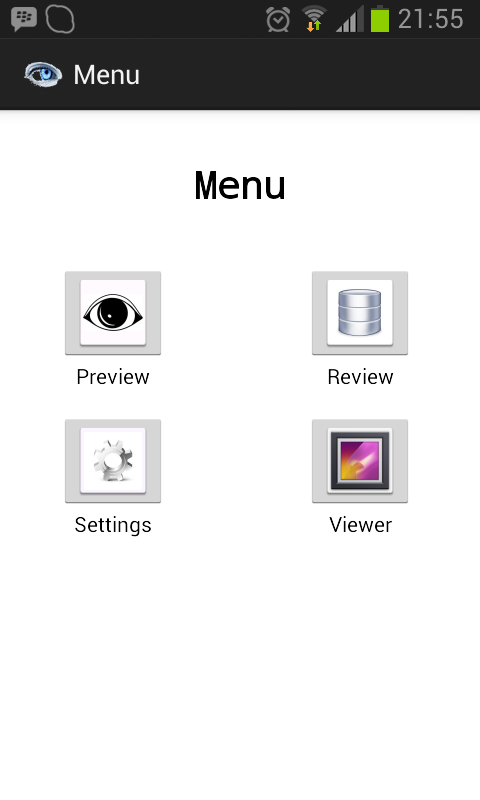
\includegraphics[width=70mm]{main.png}
\caption{Layout of Main Activity}
\label{overflow}
\end{figure}    


\subsection{Preview Activity}
The {\bf preview activity} can be regarded as the main part of this project since most of the main functionalities of the application exist here and it took 70 percent of the whole development time. This activity implements the {\bf camera preview} and sets a face detection event on each of the preview frames generated. This allows the actual real time detection, notification and logging of the events happening within this activity.

\begin{lstlisting}[label=preview-oncreate,caption=Implementation of the preview activity onCreate method] 
@Override
protected void onCreate(Bundle savedInstanceState) {
	super.onCreate(savedInstanceState);
	setContentView(R.layout.preview);

	msg = "Preview started";
	sendMsg(msg, "start");

	surfaceView = (SurfaceView) findViewById(R.id.surfaceView);
	surfaceHolder = surfaceView.getHolder();
	surfaceHolder.addCallback(this);
	surfaceHolder.setType(SurfaceHolder.SURFACE_TYPE_PUSH_BUFFERS);
	capture = (Button) findViewById(R.id.button1);
	face = (TextView) findViewById(R.id.textView1);
		
	getWindow().setFlags(WindowManager.LayoutParams.FLAG_KEEP_SCREEN_ON,
			WindowManager.LayoutParams.FLAG_KEEP_SCREEN_ON);
} 
\end{lstlisting}

The {\it onCreate()} method as discussed under activity life cycle of android application is the first method that is called when an activity is started. The implementation of the {\it onCreate()} method of the preview activity shows the instantiation of several objects, amongst which are the {\it surfaceView} and the {\it surfaceHolder} which is the surface in which the view is placed on. A callback event handler was set to the {\it surfaceHolder} on the given context so that whenever a preview frame is drawn, an implementation method of the {\it SurfaceHolder.Callback} will be executed. The surface holder type has to be set to  "SURFACE\_TYPE\_PUSH\_BUFFERS" which generates several buffers for the surface view.

For the implementation of a {\bf SurfaceHolder.Callback} implementation, there are three important methods that needs to be overridden and implemented. {\it surfaceCreated()} which is called immediately after the surface is created, {\it surfaceChanged()} is called immediately after any structural changes (format or size) have been made to the surface and {\it surfaceDestroyed()} This is called immediately before a surface is being destroyed.

\begin{lstlisting}[label=surface-created,caption=Implementation of surfaceCreated method] 
@Override
public void surfaceCreated(SurfaceHolder holder) {
	camera = Camera.open();
	if (camera != null) {
		try {
			camera.setPreviewDisplay(holder);
		} catch (Exception x) {
			camera.release();
			camera = null;
			Log.d(PreviewActivity.class.getName(),
				"Error in surface created: [" + x.getMessage() + "]");
		}
	} else
		Log.d(PreviewActivity.class.getName(), "Camera null");
}
\end{lstlisting}

Inside the surface created method, the camera instance that was created needs to be initialized (i.e opened) by calling the {\it Camera.open()} method on it and the preview display of the camera needs to be set to the surface holder that was earlier created.
\begin{lstlisting}[label=surface-changed,caption=Implementation of surfaceChanged method] 
@Override
public void surfaceChanged(SurfaceHolder holder, int format, int width,
		int height) {

	if (surfaceHolder.getSurface() == null) {
		Log.d(activityName(), "SurfaceHolder is null");
		return;
	}

	if (camera != null && !inPreview) {
		Camera.Parameters parameters = camera.getParameters();
		Camera.Size size = getPreviewSize(width, height, parameters);

		if (size != null) {
			parameters.setPreviewSize(size.width, size.height);
			camera.setParameters(parameters);
			camera.setDisplayOrientation(0);
			camera.startPreview();
			infBitmap = Bitmap.createBitmap(size.width, size.height,
					Bitmap.Config.RGB_565);
				
			inPreview = true;
			int buffSize = size.width * size.height
					* ImageFormat.getBitsPerPixel(parameters
					.getPreviewFormat()) / 8;
			byte[] Buffer = new byte[buffSize];
			camera.setPreviewCallbackWithBuffer(this);
			camera.addCallbackBuffer(Buffer);
		}

	} else
		Log.d(activityName(), "Camera null");
}  

private Camera.Size getPreviewSize(int width, int height,
			Camera.Parameters parameters) {
		Camera.Size result = null;

		for (Camera.Size size : parameters.getSupportedPreviewSizes()) {
			if (size.width <= width && size.height <= height) {
				if (result == null) {
					result = size;
				} else {
					int resultArea = result.width * result.height;
					int newArea = size.width * size.height;

					if (newArea > resultArea) {
						result = size;
					}
				}
			}
		}
		return result;
	} 
}
\end{lstlisting}	

After setting up the camera environment and display holder in the {\it surfaceCreated()} method, the next method that is on the line is the {\it surfaceChanged()} method. Within this, one has to always check if the surface holder is "null" or not, same goes to the camera instance. The parameters of the camera needs to be set by finding the best preview size possible using the {\it getPreviewSize()} method, this method goes through all the supported preview sizes checking which of the supported sizes is approximately equal to the one generated by the camera. This size's width and height is set to the parameter instance of the camera along side other configurations such as the orientation of the camera. When the camera is configured, the preview is started by calling the {\it camera.startPreview()} method. 

In the {\it surfaceChanged()} method, the buffer size of a preview frame is gotten by first creating a bitmap image with the size (width and height) of the camera preview and using a formula with the appropriate variables to calculate an approximate buffer size, the preview callback with buffer is set to this context and the buffer size is passed to the {\it camera.addCallbackBuffer()} method. This allows the method {onPreviewFrame()} method to be called and enabled to use the buffer size in generating preview frames.

\begin{lstlisting}[label=onPreview-frame,caption=Method for generating preview frames]
public void onPreviewFrame(byte[] data, Camera camera) {

	YuvImage image = new YuvImage(data, ImageFormat.NV21,
	    infBitmap.getWidth(), infBitmap.getHeight(), null);

	Rect rectangle = new Rect();
	rectangle.bottom = infBitmap.getHeight();
	rectangle.top = 0;
	rectangle.left = 0;
	rectangle.right = infBitmap.getWidth();
		
	ByteArrayOutputStream outStream;
	outStream = new ByteArrayOutputStream();
	
	stat = image.compressToJpeg(rectangle, 100, outStream);
	
	detector = new FaceDetector(infBitmap.getWidth(),
			infBitmap.getHeight(), NUM_FACES);

	BitmapFactory.Options inf = new BitmapFactory.Options();
	inf.inPreferredConfig = Bitmap.Config.RGB_565;
	bitImage = BitmapFactory.decodeStream(
	new ByteArrayInputStream(outStream.toByteArray()), null, inf);
		
	Arrays.fill(faces, null);
	facesDetected = detector.findFaces(bitImage, faces);
		
	SharedPreferences sPref;
	sPref = getSharedPreferences(PREF_NAME, 0);
		
	if(sPref.getInt("delay", 0) != 0)
		delay = sPref.getInt("delay", 30) * nanoSec;
		
	if (facesDetected > 0) {
		if (getCurrentTime() - lastTimeStamp >= delay) {
		   msg = facesDetected + " Face Detected";
		   sendMsg(msg, "face");
		   output.saveFace(bitImage);

		   email = sPref.getString("email", "nil");
		   password = sPref.getString("password", "nil");
		   phoneNumber = sPref.getString("phone", "nil");

		   if (sPref.getBoolean("emailCheck", false)) {
		      if (email == "nil" || password == "nil") {
		 	Toast.makeText(getApplicationContext(),
			"Email Settings not set ", Toast.LENGTH_SHORT)
				.show();
		       } else {
			   new Thread() {
				public void run() {
				    sendMail(email, password, output.getPath());
				}
			   }.start();
		       }
		    }

		   if (sPref.getBoolean("phoneCheck", false)) {
                          if (phoneNumber == "nil") {
		         	Toast.makeText(getApplicationContext(),
			"Phone Settings not set", Toast.LENGTH_LONG)
			.show();
		        } else {
		          	message = "Theres an intruder in your house.";
				sendSms(phoneNumber, message);
                          }
		    } else {
			Toast.makeText(getApplicationContext(),
			"Phone Settings not checked", Toast.LENGTH_LONG)
			.show();
                      }
		   lastTimeStamp = getCurrentTime();
	     }
			
	    switch (facesDetected) {
		case 1:
			face.setText(facesDetected + " Face detected");
			break;
		default:
			face.setText(facesDetected + " Faces detected");
	     }

	} else
		face.setText("No face found");

	capture.setOnClickListener(new OnClickListener() {
              @Override
	      public void onClick(View v) {
		output.saveFrame(bitImage);
		msg = "Image captured";
		sendMsg(msg, "capture");
		Toast.makeText(getApplicationContext(), "Image Captured",
				Toast.LENGTH_SHORT).show();
	      }
	});

	camera.addCallbackBuffer(data);
}
\end{lstlisting}

Listing 6.17 shows the implementation of the {\it onPreviewFrame()} method which is called whenever a preview frame is generated providing the frame as  {\it byte[]} data. This data is then converted to a YUVImage of format NV21, a rectangle is created with the size information gotten from {\it infBitmap} created in the {\it surfaceChanged()} method, a {\it ByteArrayOutputStream} instance is created and then the YUVImage is compressed as JPEG image into the outpuStream using the rectangle object that was created. With this output stream, a bitmap image is created using {\it BitmapFactory.decodeStream()} method passing the out stream which is converted to a byte array.

A {\it FaceDetector} object that was created is instantiated using the "infBitmap" information and setting the max number of faces as suited. A {\it FaceDetector.Face[]} array is then cloned using {\it Arrays.Fill()} method and initializing it to null, then faces are detected by calling {\it detector.findFaces()} passing it the parameters "bitImage" which is the bitmap image created from the data[] and "faces" which is the {\it FaceDetector.Faces[]} clone that was created, this method goes through the bitmap image, find the faces (which number is less than or equal to the maximum number of faces provided) and fill them into the faces array. 

The code that follows shows the retrieval of "email", "password" and "phone number" from shared preferences with the truth value of whether the check boxes of both email and phone notification is check, if they are, the system automatically notifies the user by both mediums using the notification module. If the value of those variables are null, that means they have not been set, the user is then notified via splash display. on click event is set on the capture button, when it is clicked, the activity uses the input output module to save the frame on the device storage drive.

\begin{lstlisting}[label=send-intent,caption=Medium to which preview activity sends messages to Logger Module]
public void sendMsg(String msg, String key) {
	Intent sendIntent = new Intent();
	sendIntent.setClass(this, LoggerService.class);
	sendIntent.putExtra(key, msg);
	startService(sendIntent);
}
\end{lstlisting} 	

The implementation of one of the ways modules communicate is by the use of {\bf intents}, listings 6.18 shows the creation of an intent, and the way message is bundled into it as "EXTRAS" and sent as a call to the method {\it startService()}.

\begin{figure}[ht!]
\centering
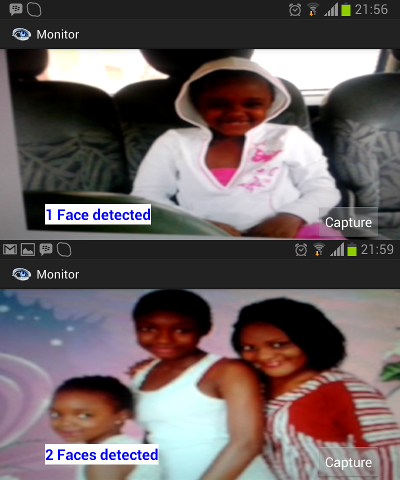
\includegraphics[width=90mm]{preview.png}
\caption{Face detection, Preview Activity}
\label{overflow}
\end{figure}    
\newpage
\subsection{Review Activity}
{\bf Review activity} is tasked with retrieving all the contents of the log(database), formatting and displaying it to the user. This activity makes use of the database module and notifier module. 

\begin{lstlisting}[label=review-oncreate,caption=Implementation of review activity onCreate() method]
@Override
protected void onCreate(Bundle savedInstanceState) {
    super.onCreate(savedInstanceState);
    setContentView(R.layout.activity_review);        
    logRecord = (TextView) findViewById(R.id.textView1);
        
    LogHelper helper = new LogHelper(this);
    log = helper.getAllEvents();
        
    sb = new StringBuilder();
    for(LogModel mod : log){
        	sb.append(mod.toString()).append("\n");
    }        
    logRecord.setText(sb.toString());
}
\end{lstlisting}

As it is for any other activity, {\it review activity} has to implement the {\it onCreate()} method. Within this method, database module is imported and an instance of "LogHelper" is created, with this log helper, the {\it LogHelper.getAllEvents()} method is called on an array list and this data in the array list is formatted by using the java "StringBuilder" after which the text is set to the display view.

The activity also provides the possibility for the user to wipe the database and to upload the log file via email using the notifier module where the java mail is implemented.

\begin{figure}[ht!]
\centering
\includegraphics[width=60mm]{Review.png}
\caption{Layout of Review Activity}
\label{overflow}
\end{figure}    

\subsection{Settings Activity}
The settings activity's task is trivial yet important. From this activity, the user information can be set and stored in the shared preferences so that other activities such as the preview and review activities can access the data and use them when notifying or uploading.

\begin{lstlisting}[label=settings-save,caption=Implementation of the settings "save" option menu]
@Override
public boolean onCreateOptionsMenu(Menu menu) {
    menu.add("Save").setOnMenuItemClickListener(
	new OnMenuItemClickListener() {

              @Override
	     public boolean onMenuItemClick(MenuItem item) {
          	SharedPreferences userData = getSharedPreferences(
			PREF_NAME, 0);

		Editor editor = userData.edit();
		editor.putString("email", email.getText().toString());
		editor.putString("password", password.getText()
				.toString());
		editor.putString("phone", phoneNo.getText().toString());
		editor.putBoolean("emailCheck", emailNotifier.isChecked());
		editor.putBoolean("phoneCheck", phoneNotifier.isChecked());
		editor.putInt("delay", Integer.parseInt(delay.getText().toString()));
		editor.commit();
		Toast.makeText(getApplicationContext(), "Data Saved",
				Toast.LENGTH_SHORT).show();
		finish();						
		return true;
	    }
         });
     return true;
}

\end{lstlisting}

The important method in the settings class worth discussing is the {\it onCreateOptionsMenu()} method. This method is mainly for creating options menu that appear when one presses the menu button on an android device, event handlers can be set to this menus and are executed when clicked on. The menu here is the "save" menu, when this menu is clicked, the values put into the entry fields are retrieved, a shared preference instance is initialized with the preference name and a space is made on the device. Each of the value retrieved from the entry fields is written into this shared preference space as a "key" and "value" pair using an "Editor" instance which writes them with the {\it Editor.put"Type"()} method, where Type can be string, integer, float e.t.c depending on the type of value. Returning true enables the use of options menu.

\begin{figure}[ht!]
\centering
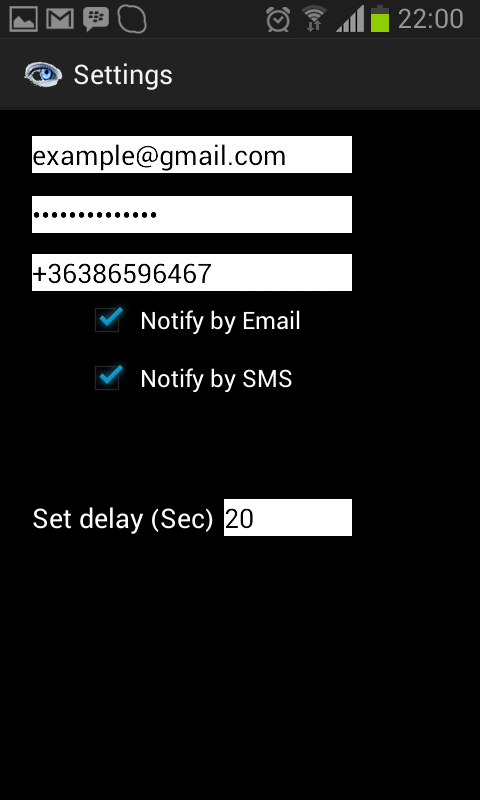
\includegraphics[width=60mm]{settings.png}
\caption{Layout of Settings Activity}
\label{overflow}
\end{figure}    
 